\documentclass[aspectratio=169, 10pt]{beamer}

% ── Base ──────────────────────────────────────────────────────────────────────
\usetheme{default}
\useinnertheme{default}
\setbeamertemplate{navigation symbols}{}

% ── Packages ──────────────────────────────────────────────────────────────────
\usepackage[T1]{fontenc}
\usepackage{lmodern}
\usepackage{microtype}
\usepackage{amsmath, amssymb}
\usepackage{booktabs}
\usepackage{xcolor}
\usepackage{tikz}
\usetikzlibrary{positioning, fit, arrows.meta, calc}
\usepackage{listings}
\usepackage{array}

% ── NYU Brand Colors (nyu.edu/brand-guidelines) ───────────────────────────────
\definecolor{Navy}    {HTML}{330662}   % Deep Violet      — dark backgrounds
\definecolor{Blue}    {HTML}{57068c}   % NYU Violet       — primary / frametitle
\definecolor{UltraV}  {HTML}{8900e1}   % Ultra Violet     — accent rule / stripe
\definecolor{MedVio}  {HTML}{702b9d}   % Medium Violet 1  — block titles
\definecolor{LightBlu}{HTML}{eee6f3}   % Light Violet 2   — block bodies
\definecolor{SlateGry}{HTML}{6d6d6d}   % Medium Gray 1    — muted text
\definecolor{OffWhite}{HTML}{f2f2f2}   % Light Gray       — code backgrounds
\definecolor{GoodGrn} {HTML}{009b8a}   % Teal             — pass / good
\definecolor{WarnRed} {HTML}{DC2626}   % Red              — warnings / fail
\definecolor{AccentYl}{HTML}{59B2D1}   % NYU Blue         — controller accent

% ── Fonts ─────────────────────────────────────────────────────────────────────
\setbeamerfont{normal text}              {family=\sffamily}
\setbeamerfont{title}                   {size=\LARGE, series=\bfseries}
\setbeamerfont{subtitle}                {size=\large,  series=\mdseries}
\setbeamerfont{frametitle}              {size=\large,  series=\bfseries}
\setbeamerfont{block title}             {size=\small,  series=\bfseries}
\setbeamerfont{block body}              {size=\small}
\setbeamerfont{itemize/enumerate body}  {size=\small}
\setbeamerfont{footline}                {size=\tiny}
\usebeamerfont{normal text}

% ── Colors ────────────────────────────────────────────────────────────────────
\setbeamercolor{normal text}   {fg=Navy}
\setbeamercolor{structure}     {fg=Blue}
\setbeamercolor{frametitle}    {fg=white, bg=Navy}
\setbeamercolor{item}          {fg=Blue}
\setbeamercolor{subitem}       {fg=SlateGry}
\setbeamercolor{block title}   {fg=white, bg=MedVio}
\setbeamercolor{block body}    {fg=Navy,  bg=OffWhite}
\setbeamercolor{alerted text}  {fg=WarnRed}
\setbeamercolor{example text}  {fg=GoodGrn}
\setbeamercolor{background canvas}{bg=white}

% ── Frametitle: navy bar + blue rule ─────────────────────────────────────────
% Note: NO \nointerlineskip — it triggers \prevdepth in horizontal mode.
% \hrule is always safe in vertical mode after a beamercolorbox.
\setbeamertemplate{frametitle}{%
  \begin{beamercolorbox}[wd=\paperwidth, ht=0.58cm, dp=0.20cm,
                          leftskip=0.40cm, rightskip=0.40cm]{frametitle}%
    \usebeamerfont{frametitle}\insertframetitle%
  \end{beamercolorbox}%
  {\color{UltraV}\hrule height 1.6pt}%
}

% ── Minimal footer ────────────────────────────────────────────────────────────
\setbeamertemplate{footline}{%
  \hfill
  \textcolor{SlateGry}{\tiny\insertframenumber\,/\,\inserttotalframenumber}%
  \hspace{6pt}\vspace{4pt}%
}

% ── Bullet style ──────────────────────────────────────────────────────────────
\setbeamertemplate{itemize item}{%
  \tikz[baseline=-0.55ex]%
    \fill[Blue] (0,0) rectangle (0.17cm,0.17cm);}
\setbeamertemplate{itemize subitem}{%
  \tikz[baseline=-0.55ex]%
    \fill[SlateGry] (0,0) circle (0.06cm);}

% ── Title page ────────────────────────────────────────────────────────────────
% Avoid beamercolorbox — its implicit bg=white covers the dark background.
\setbeamertemplate{title page}{%
  \vspace{1.7cm}
  \hspace{0.9cm}%
  \parbox[t]{0.85\paperwidth}{%
    {\color{white}\usebeamerfont{title}\inserttitle\par}%
    \vspace{0.22cm}
    {\color{white!65}\usebeamerfont{subtitle}\insertsubtitle\par}%
    \vspace{0.65cm}
    {\color{white!88}\small\insertauthor\par}%
    \vspace{0.10cm}
    {\color{white!55}\footnotesize\insertinstitute\par}%
  }%
}

% ── Helpers ───────────────────────────────────────────────────────────────────
\newcommand{\good}[1]{{\color{GoodGrn}\textbf{#1}}}
\newcommand{\warn}[1]{{\color{WarnRed}\textbf{#1}}}
\newcommand{\hl}[1]{{\color{Blue}\textbf{#1}}}
\newcommand{\muted}[1]{{\color{SlateGry}#1}}
% Horizontal rule — use \rule, never tikzpicture inline in horizontal mode
\newcommand{\hrulefull}{%
  \par\vspace{1pt}%
  {\color{SlateGry!40}\rule{\linewidth}{0.4pt}}%
  \par\vspace{2pt}%
}

% ── Code style ────────────────────────────────────────────────────────────────
\lstset{
  language=C++,
  basicstyle=\ttfamily\scriptsize\color{Navy},
  keywordstyle=\color{Blue}\bfseries,
  commentstyle=\color{SlateGry}\itshape,
  stringstyle=\color{GoodGrn},
  breaklines=true, frame=none,
  backgroundcolor=\color{OffWhite},
  xleftmargin=6pt, xrightmargin=4pt,
  aboveskip=4pt, belowskip=2pt,
}

% ── Background helper for dark slides ────────────────────────────────────────
% Usage: \darkslide{content}  — wraps with navy background + blue stripe
\newcommand{\darkslide}[1]{%
  \usebackgroundtemplate{%
    
\begin{tikzpicture}
      \fill[Navy]   (0,0) rectangle (\paperwidth,\paperheight);
      \fill[UltraV] (0,0) rectangle (\paperwidth,0.08cm);
      \fill[UltraV!35] ($(\paperwidth,\paperheight)-(1.8cm,0.6cm)$) circle (1.9cm);
      \fill[UltraV!18] ($(\paperwidth,\paperheight)-( 0.4cm,-0.2cm)$) circle (0.9cm);
    \end{tikzpicture}%
  }%
  #1%
  \usebackgroundtemplate{}%
}

% ── Meta ──────────────────────────────────────────────────────────────────────
\title{FlashAttention Accelerator on PYNQ-Z2}
\subtitle{Hardware Design --- NYU Spring 2026}
\author{Anuj Apte%
  \enspace\textbullet\enspace
  Ricardo D\'iaz%
  \enspace\textbullet\enspace
  Raquel Brown}
\institute{New York University}
\date{}

% =============================================================================
\begin{document}
% =============================================================================

% ── TITLE ────────────────────────────────────────────────────────────────────
\darkslide{%
  \begin{frame}[plain]
    \titlepage
  \end{frame}
}

% ── OUTLINE ──────────────────────────────────────────────────────────────────
\begin{frame}{Outline}
  \vspace{0.3cm}
  \begin{columns}[T]
    \begin{column}{0.44\textwidth}
      \begin{enumerate}\setlength\itemsep{8pt}
        \item \textbf{Motivation}\\
              \muted{The memory bottleneck in attention}
        \item \textbf{Algorithm}\\
              \muted{Online softmax, tiled computation}
        \item \textbf{IP Specification}\\
              \muted{Interfaces \& parameters}
      \end{enumerate}
    \end{column}
    \begin{column}{0.44\textwidth}
      \begin{enumerate}\setlength\itemsep{8pt}
        \setcounter{enumi}{3}
        \item \textbf{Architecture}\\
              \muted{7 sub-modules, HLS design}
        \item \textbf{Results}\\
              \muted{Verification \& synthesis}
        \item \textbf{Conclusions}\\
              \muted{Achievements \& next steps}
      \end{enumerate}
    \end{column}
  \end{columns}
\end{frame}

% =============================================================================
\begin{frame}{The Memory Bottleneck in Standard Attention}
% =============================================================================
  \begin{columns}[T]
    \begin{column}{0.48\textwidth}
      \vspace{0.1cm}
      Standard scaled dot-product attention:
      \[
        O = \operatorname{softmax}\!\Bigl(\tfrac{QK^T}{\sqrt{d}}\Bigr)V
      \]

      \vspace{0.05cm}
      \hrulefull

      The $N{\times}N$ score matrix $QK^T$ must be:
      \begin{itemize}\setlength\itemsep{3pt}
        \item Fully materialized before softmax
        \item Written to memory, then read back
        \item $4N^2$ bytes (float32)
      \end{itemize}

      \vspace{0.25cm}
      For $N{=}512$: score matrix $\approx \mathbf{1\,MB}$.\\[3pt]
      \warn{PYNQ-Z2 has only 140 BRAMs --- it doesn't fit.}
    \end{column}
    \begin{column}{0.48\textwidth}
      \vspace{0.1cm}
      \begin{block}{Our approach: FlashAttention}
        Process $Q$, $K$, $V$ in small tiles.\\
        Maintain running softmax state \emph{on-chip}.\\[4pt]
        \good{Peak memory: $O(N{\cdot}d)$ not $O(N^2)$}
      \end{block}

      \vspace{0.35cm}
      \begin{block}{This project}
        \begin{itemize}\setlength\itemsep{3pt}
          \item Vitis HLS implementation
          \item Target: \textbf{PYNQ-Z2} (Zynq XC7Z020)
          \item 4-channel AXI4 + AXI4-Lite control
          \item Verified against float64 golden model
        \end{itemize}
      \end{block}
    \end{column}
  \end{columns}
\end{frame}

% =============================================================================
\begin{frame}{Standard Attention --- Numerical Example ($N{=}3$, $d{=}2$)}
% =============================================================================
\begin{columns}[T]
  \begin{column}{0.50\textwidth}
    \vspace{0.05cm}
    {\small $Q = K = V = \begin{bmatrix}1&0\\0&1\\1&1\end{bmatrix}$,\quad
    $s_{ij} = \dfrac{q_i \cdot k_j}{\sqrt{2}}$}

    \vspace{0.25cm}
    \textbf{Full $3{\times}3$ score matrix} \warn{(all 9 values in memory)}

    \vspace{0.1cm}
    {\small
    \begin{tabular}{r|ccc}
         & $k_1$ & $k_2$ & $k_3$ \\\hline
    $q_1$& 0.71 & 0.00 & 0.71 \\
    $q_2$& 0.00 & 0.71 & 0.71 \\
    $q_3$& 0.71 & 0.71 & 1.41 \\
    \end{tabular}
    }

    \vspace{0.25cm}
    \textbf{Softmax row $q_1$:}\\[3pt]
    {\small
    $e^{[0.71,\;0.00,\;0.71]-0.71} = [1.00,\;0.49,\;1.00]$\\[2pt]
    $\ell = 2.49 \;\Rightarrow\; p_1 = [0.40,\;0.20,\;0.40]$\\[4pt]
    $o_1 = p_1 \cdot V = \good{[0.80,\;0.60]}$
    }
  \end{column}
  \begin{column}{0.46\textwidth}
    \vspace{0.1cm}
    \textbf{All $N^2{=}9$ scores in memory at once}
    \vspace{0.15cm}

    \centering
    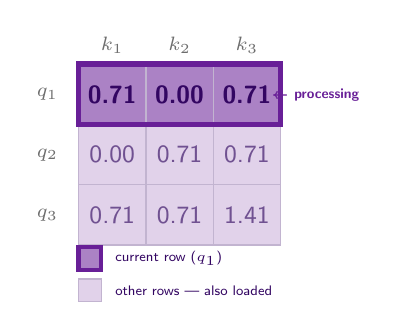
\begin{tikzpicture}[scale=0.90]
      % ── background: all cells in memory ─────────────────────────────────────
      \foreach \i in {0,...,2} { \foreach \j in {0,...,2} {
        \fill[Blue!18] (\j*0.95, -\i*0.85) rectangle ++(0.95,0.85);
      }}
      % ── highlight q1 row (current row being processed) ───────────────────────
      \foreach \j in {0,...,2} {
        \fill[Blue!50] (\j*0.95, 0) rectangle ++(0.95,0.85);
      }
      % ── cell grid ────────────────────────────────────────────────────────────
      \foreach \i in {0,...,2} { \foreach \j in {0,...,2} {
        \draw[Navy!30, line width=0.5pt] (\j*0.95, -\i*0.85) rectangle ++(0.95,0.85);
      }}
      % ── thick border around q1 row ───────────────────────────────────────────
      \draw[Blue!90, line width=2.0pt] (0, 0) rectangle ++(2.85, 0.85);
      % ── score values in all cells ────────────────────────────────────────────
      \foreach \j/\v in {0/0.71, 1/0.00, 2/0.71} {
        \node[font=\small\sffamily\bfseries, text=Navy]
          at (\j*0.95+0.475, 0.42) {\v};
      }
      \foreach \j/\v in {0/0.00, 1/0.71, 2/0.71} {
        \node[font=\small\sffamily, text=Navy!70]
          at (\j*0.95+0.475, -0.43) {\v};
      }
      \foreach \j/\v in {0/0.71, 1/0.71, 2/1.41} {
        \node[font=\small\sffamily, text=Navy!70]
          at (\j*0.95+0.475, -1.28) {\v};
      }
      % ── row label above highlighted row ──────────────────────────────────────
      \node[font=\tiny\sffamily\bfseries, text=Blue!90]
        at (3.35, 0.42) {← processing};
      % ── axis labels ───────────────────────────────────────────────────────────
      \foreach \j/\lab in {0/$k_1$, 1/$k_2$, 2/$k_3$} {
        \node[font=\scriptsize\sffamily, text=SlateGry]
          at (\j*0.95+0.475, 1.12) {\lab};
      }
      \foreach \i/\lab in {0/$q_1$, 1/$q_2$, 2/$q_3$} {
        \node[font=\scriptsize\sffamily, text=SlateGry]
          at (-0.44, -\i*0.85+0.42) {\lab};
      }
      % ── legend ───────────────────────────────────────────────────────────────
      \fill[Blue!50] (0,-2.05) rectangle ++(0.32,0.32);
      \draw[Blue!90, line width=1.5pt] (0,-2.05) rectangle ++(0.32,0.32);
      \node[font=\tiny\sffamily, right, text=Navy] at (0.38,-1.89) {current row ($q_1$)};
      \fill[Blue!18] (0,-2.50) rectangle ++(0.32,0.32);
      \draw[Navy!30, line width=0.5pt] (0,-2.50) rectangle ++(0.32,0.32);
      \node[font=\tiny\sffamily, right, text=Navy] at (0.38,-2.34) {other rows — also loaded};
    \end{tikzpicture}

    \vspace{0.15cm}
    \raggedright
    \warn{Softmax needs all 9 scores before\\it can compute a single probability.}
  \end{column}
\end{columns}
\end{frame}

% =============================================================================
\begin{frame}{FlashAttention --- Same Example, $B_Q{=}B_K{=}2$}
% =============================================================================
\begin{columns}[T]
  \begin{column}{0.52\textwidth}
    \vspace{0.05cm}
    {\small Focus on row $q_1{=}[1,0]$. Init: $m{=}{-\infty}$, $\ell{=}0$, $o{=}[0,0]$.}

    \vspace{0.2cm}
    \textbf{K/V tile 0} \muted{($k_1,k_2$ on-chip)}
    {\small
    \begin{itemize}\setlength\itemsep{1pt}
      \item Scores: $[0.71,\;0.00]$
      \item $m \leftarrow 0.71$,\quad $e^{s-m}{=}[1.00,\;0.49]$
      \item $\ell \leftarrow 1.49$
      \item $o \leftarrow \tfrac{1.00\cdot[1,0]+0.49\cdot[0,1]}{1.49} = [0.67,\;0.33]$
    \end{itemize}
    }

    \vspace{0.15cm}
    \textbf{K/V tile 1} \muted{($k_3$ on-chip)}
    {\small
    \begin{itemize}\setlength\itemsep{1pt}
      \item Score: $[0.71]$\quad ($m$ unchanged $\Rightarrow$ correction $c{=}1$)
      \item $\ell \leftarrow 1\cdot1.49 + 1.00 = 2.49$
      \item $o \leftarrow \tfrac{1\cdot1.49\cdot[0.67,0.33]+1.00\cdot[1,1]}{2.49}$\\[2pt]
            $\phantom{o \leftarrow} = \good{[0.80,\;0.60]}$ \quad\good{\checkmark same answer}
    \end{itemize}
    }

    \vspace{0.1cm}
    \good{Max on-chip at once: $1{\times}2 = 2$ scores.}\\
    \good{Full $3{\times}3$ matrix never materializes.}
  \end{column}
  \begin{column}{0.44\textwidth}
    \vspace{0.1cm}
    \textbf{$3{\times}3$ score space — Q tile 0 ($q_1, q_2$)}
    \vspace{0.15cm}

    \centering
    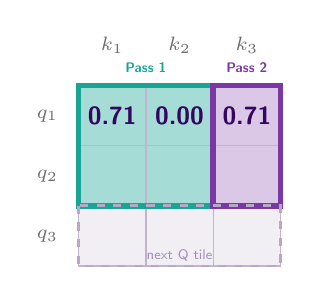
\begin{tikzpicture}[scale=0.90]
      % ── background cells ────────────────────────────────────────────────────
      \foreach \i in {0,...,2} {
        \foreach \j in {0,...,2} {
          \fill[Navy!7] (\j*0.95, -\i*0.85) rectangle ++(0.95,0.85);
        }
      }
      % ── tile fills (draw before borders) ────────────────────────────────────
      % Pass 1 (green): top-left 2×2
      \foreach \i in {0,1} { \foreach \j in {0,1} {
        \fill[GoodGrn!35] (\j*0.95, -\i*0.85) rectangle ++(0.95,0.85);
      }}
      % Pass 2 (blue): top-right 2×1
      \foreach \i in {0,1} {
        \fill[Blue!22] (1.90, -\i*0.85) rectangle ++(0.95,0.85);
      }
      % ── cell grid ────────────────────────────────────────────────────────────
      \foreach \i in {0,...,2} { \foreach \j in {0,...,2} {
        \draw[Navy!30, line width=0.5pt] (\j*0.95, -\i*0.85) rectangle ++(0.95,0.85);
      }}
      % ── thick tile borders ────────────────────────────────────────────────────
      % Pass 1 border
      \draw[GoodGrn!90, line width=2.0pt] (0, 0.85) rectangle ++(1.90,-1.70);
      % Pass 2 border
      \draw[Blue!80, line width=2.0pt] (1.90, 0.85) rectangle ++(0.95,-1.70);
      % Q tile 1 border (next Q tile, not computed yet)
      \draw[Navy!35, line width=1.0pt, dashed] (0,-0.85) rectangle ++(2.85,-0.85);

      % ── pass labels above tiles ───────────────────────────────────────────────
      \node[font=\tiny\sffamily\bfseries, text=GoodGrn!90]
        at (0.95, 1.10) {Pass 1};
      \node[font=\tiny\sffamily\bfseries, text=Blue!80]
        at (2.375, 1.10) {Pass 2};
      \node[font=\tiny\sffamily, text=Navy!45]
        at (1.425, -1.55) {next Q tile};

      % ── score values for q1 row ───────────────────────────────────────────────
      \foreach \j/\v in {0/0.71, 1/0.00, 2/0.71} {
        \node[font=\small\sffamily\bfseries, text=Navy]
          at (\j*0.95+0.475, 0.42) {\v};
      }

      % ── axis labels ───────────────────────────────────────────────────────────
      \foreach \j/\lab in {0/$k_1$, 1/$k_2$, 2/$k_3$} {
        \node[font=\scriptsize\sffamily, text=SlateGry]
          at (\j*0.95+0.475, 1.42) {\lab};
      }
      \foreach \i/\lab in {0/$q_1$, 1/$q_2$, 2/$q_3$} {
        \node[font=\scriptsize\sffamily, text=SlateGry]
          at (-0.44, -\i*0.85+0.42) {\lab};
      }
    \end{tikzpicture}

    \vspace{0.15cm}
    \raggedright
    {\small Numbers shown are $q_1$'s scores per tile.\\
    Each pass loads only one K/V tile at a time.}
  \end{column}
\end{columns}
\end{frame}

% =============================================================================
\begin{frame}{Online Softmax: Exact Attention Without the Full Matrix}
% =============================================================================
  \begin{columns}[T]
    \begin{column}{0.46\textwidth}
      \textbf{State per query row $i$ (lives on-chip):}
      \begin{itemize}\setlength\itemsep{2pt}
        \item $m_i$ --- running row maximum
        \item $l_i$ --- running normalization sum
        \item $o_i$ --- running output accumulator
      \end{itemize}

      \vspace{0.25cm}
      \textbf{Per K/V tile update:}
      \vspace{0.1cm}

      {\small
        $m_i^{\mathrm{new}} = \max\!\bigl(m_i,\;\max_j s_{ij}\bigr)$
        \par\vspace{4pt}
        $l_i^{\mathrm{new}} = \underbrace{e^{m_i - m_i^{\mathrm{new}}}}_{\text{correction }c}
          l_i + \textstyle\sum_j e^{s_{ij} - m_i^{\mathrm{new}}}$
        \par\vspace{4pt}
        $o_i^{\mathrm{new}} =
          \dfrac{c\,l_i\,o_i +
                 \sum_j e^{s_{ij}-m_i^{\mathrm{new}}} v_j}
                {l_i^{\mathrm{new}}}$
      }

      \vspace{0.25cm}
      \good{$o_i$ stays normalized after every tile.}\\
      \good{No final division needed.}
    \end{column}
    \begin{column}{0.50\textwidth}
      \begin{block}{Algorithm (BQ = BK = 8)}
        \vspace{2pt}
        {\ttfamily\scriptsize\color{Navy}
          \textbf{for} q0 in 0, BQ, 2$\times$BQ, \ldots, N:\\
          \quad load Q tile \hfill\textit{(8 rows)}\\
          \quad init $m\!=\!-\infty$, $l\!=\!0$, $o\!=\!0$\\[3pt]
          \quad\textbf{for} k0 in 0, BK, 2$\times$BK, \ldots, N:\\
          \quad\quad load K, V tiles\\
          \quad\quad scores $= Q_t K_t^T / \sqrt{d}$\\
          \quad\quad apply causal mask if needed\\
          \quad\quad update $m$, $l$, $o$ online\\[3pt]
          \quad write output tile
        }
        \vspace{2pt}
      \end{block}

      \vspace{0.3cm}
      \begin{itemize}\setlength\itemsep{3pt}
        \item Correction $c\!=\!e^{m_i-m_i^{\mathrm{new}}}$ rescales prior
              state when max grows
        \item Causal mask: $s_{ij}\!=\!-10^{30}$ for $j{>}i$,
              so $e^{s_{ij}}\!\to\!0$ with no extra branch
      \end{itemize}
    \end{column}
  \end{columns}
\end{frame}

% =============================================================================
\begin{frame}{IP Specification}
% =============================================================================
  \begin{columns}[T]
    \begin{column}{0.38\textwidth}
      \begin{block}{Compile-time limits}
        \vspace{2pt}
        \begin{tabular}{lrl}
          \texttt{N\_MAX} & 64 & max seq length \\
          \texttt{D\_MAX} & 32 & max dimension  \\
          \texttt{BQ}     &  8 & Q tile size    \\
          \texttt{BK}     &  8 & K/V tile size  \\
        \end{tabular}
        \vspace{2pt}
      \end{block}

      \vspace{0.3cm}
      \begin{block}{Runtime (AXI4-Lite regs)}
        \vspace{2pt}
        \begin{tabular}{ll}
          \texttt{N}       & sequence length \\
          \texttt{d}       & embedding dim   \\
          \texttt{causal}  & 0 or 1          \\
          Q/K/V/O addr     & 64-bit DDR ptr  \\
        \end{tabular}
        \vspace{2pt}
      \end{block}
    \end{column}
    \begin{column}{0.58\textwidth}
      \vspace{0.1cm}
      \textbf{Hardware / Software boundary}
      \hrulefull
      \begin{itemize}\setlength\itemsep{4pt}
        \item \textbf{PS (ARM):} allocates DDR buffers; writes parameters
              to AXI4-Lite registers; asserts \texttt{AP\_START};
              polls \texttt{AP\_DONE}
        \item \textbf{PL (this IP):} reads tiles via AXI4 Master,
              computes on-chip, writes $O$ back to DDR
        \item Intermediate state ($m$, $l$, scores, acc)
              \emph{never} leaves the chip
      \end{itemize}

      \vspace{0.25cm}
      \textbf{AXI4 Master channels} \muted{(no DDR contention)}

      \vspace{0.1cm}
      \begin{tabular}{llll}
        \texttt{gmem0} & $Q$ & read  & 32-bit / 16-burst \\
        \texttt{gmem1} & $K$ & read  & 32-bit / 16-burst \\
        \texttt{gmem2} & $V$ & read  & 32-bit / 16-burst \\
        \texttt{gmem3} & $O$ & write & 32-bit / 16-burst \\
      \end{tabular}
    \end{column}
  \end{columns}
\end{frame}

% =============================================================================
\begin{frame}{Architecture Overview}
% =============================================================================
\vspace{-0.1cm}
\centering
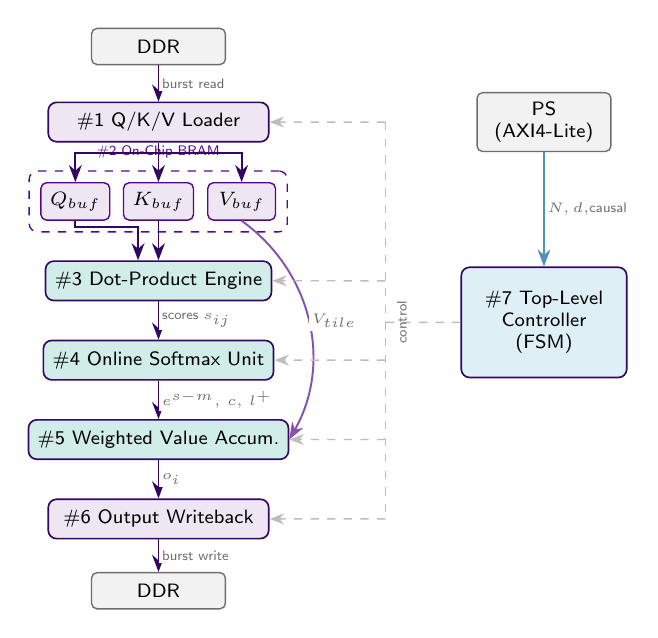
\begin{tikzpicture}[
  font=\scriptsize\sffamily, >=Stealth,
  every node/.style={align=center},
  mem/.style    = {draw=Navy, fill=LightBlu, rounded corners=3pt,
                   minimum width=2.8cm, minimum height=0.50cm, line width=0.6pt},
  compute/.style= {draw=Navy, fill=GoodGrn!18, rounded corners=3pt,
                   minimum width=2.8cm, minimum height=0.50cm, line width=0.6pt},
  ext/.style    = {draw=SlateGry, fill=OffWhite, rounded corners=2pt,
                   minimum width=1.7cm, minimum height=0.46cm, line width=0.5pt},
  ctrl/.style   = {draw=Navy, fill=AccentYl!20, rounded corners=3pt,
                   minimum width=2.1cm, minimum height=1.4cm, line width=0.6pt},
  buf/.style    = {draw=Blue, fill=LightBlu, rounded corners=2pt,
                   minimum width=0.86cm, minimum height=0.44cm, line width=0.5pt},
  sig/.style    = {font=\tiny\sffamily, fill=white, inner sep=1pt, text=SlateGry},
  scale=0.96,
]
\node[ext]     (ddr_r) at (0,   0   ) {DDR};
\node[mem]     (loader)at (0,  -1.0 ) {\#1 Q/K/V Loader};
\node[buf]     (qbuf)  at (-1.1,-2.05) {$Q_{buf}$};
\node[buf]     (kbuf)  at (  0, -2.05) {$K_{buf}$};
\node[buf]     (vbuf)  at ( 1.1,-2.05) {$V_{buf}$};
\node[draw=Blue, dashed, rounded corners=3pt, inner sep=4pt, line width=0.5pt,
      fit=(qbuf)(kbuf)(vbuf),
      label={[font=\tiny\sffamily,text=Blue,yshift=1pt]above:\#2 On-Chip BRAM}]{};
\node[compute] (dp)    at (0,  -3.1 ) {\#3 Dot-Product Engine};
\node[compute] (sfx)   at (0,  -4.15) {\#4 Online Softmax Unit};
\node[compute] (acc)   at (0,  -5.2 ) {\#5 Weighted Value Accum.};
\node[mem]     (wb)    at (0,  -6.25) {\#6 Output Writeback};
\node[ext]     (ddr_w) at (0,  -7.2 ) {DDR};
\node[ext]  (ps)  at (5.1, -1.0 ) {PS\\(AXI4-Lite)};
\node[ctrl] (ctl) at (5.1, -3.65) {\#7 Top-Level\\Controller\\(FSM)};

\draw[->,line width=0.7pt,Navy] (ddr_r) -- node[sig,right]{burst read}  (loader);
\draw[->,line width=0.7pt,Navy] (loader.south) -- ++(0,-0.14) -| (qbuf.north);
\draw[->,line width=0.7pt,Navy] (loader.south) -- ++(0,-0.14) -- (kbuf.north);
\draw[->,line width=0.7pt,Navy] (loader.south) -- ++(0,-0.14) -| (vbuf.north);
\draw[->,line width=0.7pt,Navy] (qbuf.south) -- ++(0,-0.08) -| ([xshift=-0.27cm]dp.north);
\draw[->,line width=0.7pt,Navy] (kbuf.south) -- (dp.north);
\draw[->,bend left=42,line width=0.7pt,Blue!70]
      (vbuf.south) to node[sig,pos=0.5,right]{$V_{tile}$} (acc.east);
\draw[->,line width=0.7pt,Navy] (dp)  -- node[sig,right]{scores $s_{ij}$}        (sfx);
\draw[->,line width=0.7pt,Navy] (sfx) -- node[sig,right]{$e^{s-m},\,c,\,l^{+}$} (acc);
\draw[->,line width=0.7pt,Navy] (acc) -- node[sig,right]{$o_i$}                   (wb);
\draw[->,line width=0.7pt,Navy] (wb)  -- node[sig,right]{burst write}              (ddr_w);
\draw[->,line width=0.7pt,AccentYl!80!Navy]
      (ps) -- node[sig,right]{$N,d,$causal} (ctl);
\coordinate (bt) at (3.0,-1.0);
\coordinate (bb) at (3.0,-6.25);
\draw[SlateGry!45,dashed,line width=0.5pt] (ctl.west) -- (3.0,-3.65);
\draw[SlateGry!45,dashed,line width=0.5pt] (bt) -- (bb);
\foreach \y/\m in {-1.0/loader,-3.1/dp,-4.15/sfx,-5.2/acc,-6.25/wb}{
  \draw[->,SlateGry!45,dashed,line width=0.5pt] (3.0,\y) -- (\m.east);
}
\node[rotate=90,font=\tiny\sffamily,text=SlateGry] at (3.22,-3.65){control};
\end{tikzpicture}
\end{frame}

% =============================================================================
\begin{frame}[fragile]{HLS Implementation Highlights}
% =============================================================================
  \begin{columns}[T]
    \begin{column}{0.50\textwidth}
      \textbf{Dot-product engine: II = 1 via full unroll}
      \vspace{2pt}
      \begin{lstlisting}
SCORE_LOOP_J:
for (int j = 0; j < k_lim; j++) {
#pragma HLS PIPELINE II=1
  data_t dot = 0.0f;
  for (int x = 0; x < D_MAX; x++) {
#pragma HLS UNROLL   // 32 parallel MACs
    if (x < d) dot += Qbuf[i][x]*Kbuf[j][x];
  }
  float s = dot * inv_sqrt_d;
  // causal: exp(-1e30) -> 0, no branch in softmax
  if (causal && (k0+j) > (q0+i)) s = -1e30f;
  scores[i][j] = s;
}
      \end{lstlisting}
      \vspace{4pt}
      \textbf{BRAM partitioned for 4-wide parallel reads}
      \begin{lstlisting}
#pragma HLS ARRAY_PARTITION \
        variable=Qbuf cyclic factor=4 dim=2
#pragma HLS ARRAY_PARTITION \
        variable=Kbuf cyclic factor=4 dim=2
      \end{lstlisting}
    \end{column}
    \begin{column}{0.46\textwidth}
      \begin{block}{All inner loops: II = 1}
        \vspace{2pt}
        \begin{tabular}{lrr}
          \toprule
          Loop         & II & Latency \\
          \midrule
          LOAD\_Q      &  1 & 12 cyc \\
          LOAD\_KV     &  1 & 12 cyc \\
          SCORE\_LOOP  &  1 & 202 cyc \\
          FIND\_MAX    &  1 &  3 cyc \\
          UPDATE\_ACC  &  1 & 34 cyc \\
          STORE\_O     &  1 &  9 cyc \\
          \bottomrule
        \end{tabular}
        \vspace{2pt}
      \end{block}

      \vspace{0.15cm}
      \begin{block}{Interface notes}
        \vspace{2pt}
        \begin{itemize}\setlength\itemsep{1pt}
          \item \texttt{float *Q} (1D) for AXI4 Master — 2D arrays unsynthesizable
          \item \texttt{int causal} not \texttt{bool} — 32-bit AXI4-Lite register
          \item \texttt{hls::expf}/\texttt{sqrtf} — synthesizable math
        \end{itemize}
        \vspace{2pt}
      \end{block}
    \end{column}
  \end{columns}
\end{frame}

% =============================================================================
\begin{frame}{Functional Verification --- Testbench}
% =============================================================================
  \begin{columns}[T]
    \begin{column}{0.56\textwidth}
      \textbf{Testbench pipeline}
      \hrulefull
      \begin{enumerate}\setlength\itemsep{3pt}
        \item Python golden model generates vectors in \textbf{float64}
        \item CSV loaded by C++ testbench (1D arrays, D\_MAX stride)
        \item \texttt{flash\_attention\_hls()} called in\\
              C-sim \emph{and} RTL co-simulation identically
        \item Max absolute error reported per test
      \end{enumerate}
    \end{column}
    \begin{column}{0.40\textwidth}
      \textbf{Coverage}
      \hrulefull
      \begin{itemize}\setlength\itemsep{3pt}
        \item Single-tile ($N \le 8$)
        \item Multi-tile ($N{=}16$, $N{=}32$)
        \item \hl{Partial tile} ($N{=}13$,\\
              q\_lim $=$ k\_lim $=$ 5)
        \item Max size ($N{=}64$, $d{=}32$)
        \item Full and causal masking
        \item Verified in Vitis HLS\\(C-sim \& RTL co-sim)
      \end{itemize}
    \end{column}
  \end{columns}
\end{frame}

% =============================================================================
\begin{frame}{Functional Verification --- Results}
% =============================================================================
  \vspace{0.1cm}
  \begin{columns}[T]
    \begin{column}{0.60\textwidth}
      \textbf{Per-test results} \quad \muted{(Vitis HLS C-sim \& RTL co-sim, tolerance $= 10^{-4}$)}
      \vspace{0.15cm}

      {\small
      \begin{tabular}{ccclr}
        \toprule
        ID & $N$ & $d$ & Causal & Max $|$err$|$ vs float64 \\
        \midrule
        0 & 4  & 4  & No  & $6.0\times10^{-8}$\quad\good{\checkmark} \\
        1 & 4  & 4  & Yes & $1.2\times10^{-7}$\quad\good{\checkmark} \\
        2 & 8  & 4  & Yes & $1.2\times10^{-7}$\quad\good{\checkmark} \\
        3 & 16 & 8  & No  & $2.1\times10^{-7}$\quad\good{\checkmark} \\
        4 & 16 & 8  & Yes & $1.2\times10^{-7}$\quad\good{\checkmark} \\
        5 & 13 & 8  & No  & $3.6\times10^{-7}$\quad\good{\checkmark} \\
        6 & 13 & 8  & Yes & $2.4\times10^{-7}$\quad\good{\checkmark} \\
        7 & 32 & 16 & No  & $1.8\times10^{-7}$\quad\good{\checkmark} \\
        8 & 64 & 32 & No  & $3.0\times10^{-7}$\quad\good{\checkmark} \\
        \bottomrule
      \end{tabular}
      }
    \end{column}
    \begin{column}{0.36\textwidth}
      \begin{block}{\good{9 / 9 PASS}}
        \vspace{2pt}
        Max error $\mathbf{3.6\times10^{-7}}$\\[3pt]
        $270\times$ below $10^{-4}$ tol.\\[3pt]
        C-sim and RTL co-sim\\results are identical.
        \vspace{2pt}
      \end{block}
      \vspace{0.3cm}
      \muted{\small Test 5 (N=13) is the worst case — partial tile boundary where the last Q and K tiles are only 5 rows wide.}
    \end{column}
  \end{columns}
\end{frame}

% =============================================================================
\begin{frame}{Synthesis Results --- PYNQ-Z2 (XC7Z020, 100 MHz)}
% =============================================================================
  \begin{columns}[T]
    \begin{column}{0.46\textwidth}
      \begin{block}{Resource Utilization}
        \vspace{2pt}
        \begin{tabular}{lrrr}
          \toprule
          Resource    & Used    & Avail    & \%  \\
          \midrule
          BRAM\_18K   & 141     & 280      & 50\% \\
          DSP48E1     & 178     & 220      & \warn{81\%} \\
          Flip-Flops  & 31\,527 & 106\,400 & 30\% \\
          LUTs        & 40\,259 &  53\,200 & \warn{76\%} \\
          \bottomrule
        \end{tabular}
        \vspace{2pt}
      \end{block}

      \vspace{0.25cm}
      \textbf{Key driver:} 32 fully-unrolled MACs\\
      consume \textbf{141 of 178 DSPs}.\\[4pt]
      Switching to \texttt{ap\_fixed<16,6>}\\
      would cut DSP usage significantly.
    \end{column}
    \begin{column}{0.50\textwidth}
      \begin{block}{Timing}
        \vspace{2pt}
        \begin{tabular}{ll}
          \toprule
          Metric        & Value \\
          \midrule
          Target clock  & 10 ns (100 MHz) \\
          Timing slack  & \warn{$-1.40$ ns} \\
          Critical path & FIND\_MAX chain  \\
          Est.\ max freq & $\approx 87$ MHz \\
          \bottomrule
        \end{tabular}
        \vspace{2pt}
      \end{block}

      \vspace{0.25cm}
      \begin{block}{AXI4 burst inference}
        \vspace{2pt}
        \begin{itemize}\setlength\itemsep{2pt}
          \item All 4 M\_AXI ports: \good{burst inferred}
          \item Variable-length, up to tile size
          \item 4 separate DDR channels = no contention
        \end{itemize}
        \vspace{2pt}
      \end{block}
    \end{column}
  \end{columns}
\end{frame}

% =============================================================================
\begin{frame}{Conclusions \& Future Work}
% =============================================================================
  \begin{columns}[T]
    \begin{column}{0.48\textwidth}
      \begin{block}{\good{Delivered}}
        \vspace{2pt}
        \begin{itemize}\setlength\itemsep{3pt}
          \item Full FlashAttention forward pass, Vitis HLS
          \item PYNQ-Z2 (XC7Z020) --- PS-ready IP block
          \item 4-channel AXI4 Master + AXI4-Lite control
          \item All inner loops: \good{II = 1}
          \item \good{9/9 tests pass} in Vitis HLS (C-sim \& RTL co-sim)
          \item Max error: $3.6\times10^{-7}$
                ($270\times$ below tolerance)
          \item Optional causal masking at no latency cost
        \end{itemize}
        \vspace{2pt}
      \end{block}
    \end{column}
    \begin{column}{0.48\textwidth}
      \begin{block}{Next steps}
        \vspace{2pt}
        \begin{itemize}\setlength\itemsep{2pt}
          \item Registered FIND\_MAX tree $\to$ fix timing
          \item \texttt{\#pragma HLS DATAFLOW} $\to$\\
                overlap load / compute / store
          \item \texttt{ap\_fixed<16,6>} $\to$ cut DSPs,\\
                quantify accuracy tradeoff
          \item Multi-head via time-multiplexing
        \end{itemize}
        \vspace{2pt}
      \end{block}
    \end{column}
  \end{columns}
\end{frame}

% ── CLOSING ───────────────────────────────────────────────────────────────────
\darkslide{%
  \begin{frame}[plain]
    \centering
    \vspace{3.2cm}
    {\color{white}\LARGE\bfseries Thank you}\\[0.5cm]
    {\color{white!70}\large Questions?}\\[0.8cm]
    {\color{white!60}\small
      Anuj Apte\enspace$\cdot$\enspace
      Ricardo D\'iaz\enspace$\cdot$\enspace
      Raquel Brown}\\[0.2cm]
    {\color{UltraV!80}\footnotesize\ttfamily
      github.com/ricardotk002/hwdesign-flash-attn-accel}
  \end{frame}
}

\end{document}
